% Format teze zasnovan je na paketu memoir
% http://tug.ctan.org/macros/latex/contrib/memoir/memman.pdf ili
% http://texdoc.net/texmf-dist/doc/latex/memoir/memman.pdf
% 
% Prilikom zadavanja klase memoir, navedenim opcijama se podešava 
% veličina slova (12pt) i jednostrano štampanje (oneside).
% Ove parametre možete menjati samo ako pravite nezvanične verzije
% mastera za privatnu upotrebu (na primer, u b5 varijanti ima smisla 
% smanjiti 
\documentclass[12pt,oneside]{memoir} 

% Paket koji definiše sve specifičnosti master rada Matematičkog fakulteta
\usepackage[latinica]{matfmaster} 

\usepackage[bottom]{footmisc}
\usepackage{latexsym}
\usepackage{amssymb}
\usepackage{amsmath}
\usepackage{algorithm}
\usepackage{algpseudocode}
\usepackage{listings}
\usepackage{bm}



% Define a custom color
\definecolor{backcolour}{rgb}{0.95,0.95,0.92}
\definecolor{codegreen}{rgb}{0,0.6,0}

% Define a custom style
\lstdefinestyle{myStyle}{
    backgroundcolor=\color{backcolour},   
    commentstyle=\color{codegreen},
    basicstyle=\ttfamily\footnotesize,
    breakatwhitespace=false,         
    breaklines=true,                 
    keepspaces=true,                 
    numbers=left,       
    numbersep=5pt,                  
    showspaces=false,                
    showstringspaces=false,
    showtabs=false,                  
    tabsize=2,
}

% Use \lstset to make myStyle the global default
\lstset{style=myStyle}

\makeatletter
\renewcommand{\ALG@name}{Algoritam}
\makeatother
%
% Podrazumevano pismo je ćirilica.
%   Ako koristite pdflatex, a ne xetex, sav latinički tekst na srpskom jeziku
%   treba biti okružen sa \lat{...} ili \begin{latinica}...\end{latinica}.
%
% Opicija [latinica]:
%   ako želite da pišete latiniciom, dodajte opciju "latinica" tj.
%   prethodni paket uključite pomoću: \usepackage[latinica]{matfmaster}.
%   Ako koristite pdflatex, a ne xetex, sav ćirilički tekst treba biti
%   okružen sa \cir{...} ili \begin{cirilica}...\end{cirilica}.
%
% Opcija [biblatex]:
%   ako želite da koristite reference na više jezika i umesto paketa
%   bibtex da koristite BibLaTeX/Biber, dodajte opciju "biblatex" tj.
%   prethodni paket uključite pomoću: \usepackage[biblatex]{matfmaster}
%
% Opcija [b5paper]:
%   ako želite da napravite verziju teze u manjem (b5) formatu, navedite
%   opciju "b5paper", tj. prethodni paket uključite pomoću: 
%   \usepackage[b5paper]{matfmaster}. Tada ima smisla razmisliti o promeni
%   veličine slova (izmenom opcije 12pt na 11pt u \documentclass{memoir}).
%
% Naravno, opcije je moguće kombinovati.
% Npr. \usepackage[b5paper,biblatex]{matfmaster}

% Pomoćni paket koji generiše nasumičan tekst u kojem se javljaju sva slova
% azbuke (nema potrebe koristiti ovo u pravim disertacijama)
\usepackage[latinica]{pangrami}

% Datoteka sa literaturom u BibTex tj. BibLaTeX/Biber formatu
\bib{matfmaster-primer}

% Ime kandidata na srpskom jeziku (u odabranom pismu)
\autor{Miloš P. Miković}
% Naslov teze na srpskom jeziku (u odabranom pismu)
\naslov{Algoritmi za rešavanje problema najkraće zajedničke nadniske}
% Godina u kojoj je teza predana komisiji
\godina{2021}
% Ime i afilijacija mentora (u odabranom pismu)
\mentor{dr Aleksandar \textsc{Kartelj}, docent\\ Univerzitet u Beogradu, Matematički fakultet}
% Ime i afilijacija prvog člana komisije (u odabranom pismu)
\komisijaA{dr Vladimir \textsc{Filipović}, redovni profesor\\ Univerzitet u Beogradu, Matematički fakultet}
% Ime i afilijacija drugog člana komisije (u odabranom pismu)
\komisijaB{dr Stefan \textsc{Mišković}, docent\\ Univerzitet u Beogradu, Matematički fakultet}
% Ime i afilijacija trećeg člana komisije (opciono)
% \komisijaC{}
% Ime i afilijacija četvrtog člana komisije (opciono)
% \komisijaD{}
% Datum odbrane (odkomentarisati narednu liniju i upisati datum odbrane ako je poznat)
% \datumodbrane{}

% Apstrakt na srpskom jeziku (u odabranom pismu)
\apstr{%
% \pangrami
}

% Ključne reči na srpskom jeziku (u odabranom pismu)
\kljucnereci{optimizacija, pretraga bima, analiza bioloških sekvenci}

\begin{document}
% ==============================================================================
% Uvodni deo teze
\frontmatter
% ==============================================================================
% Naslovna strana
\naslovna
% Strana sa podacima o mentoru i članovima komisije
\komisija
% Strana sa posvetom (u odabranom pismu)
\posveta{Hvala profesoru Aleksandru Kartelju.}
% Strana sa podacima o disertaciji na srpskom jeziku
\apstrakt
% Sadržaj teze
\tableofcontents*

% ==============================================================================
% Glavni deo teze
\mainmatter
% ==============================================================================

% ------------------------------------------------------------------------------
\chapter{Uvod}
% ------------------------------------------------------------------------------
% \pangrami
Problem najkraće zajedničke nadniske (\textit{eng.} Shortest Common Supersequence Problem)
jedan je od dobro poznatih NP-teških problema optimizacije u oblasti analize reči \cite{ProbabilisticBS}.
Ukratko, PNZN\footnote{U nastavku teksta PNZN ćemo koristiti kao skraćenicu za problem najkraće zajedničke nadniske}
se može opisati kao problem pronalaženja najkraće reči $\omega$ sačinjene
od simbola zadate konačne Azbuke $\Sigma$, tako da su sve sekvence iz unapred zadatog konačnog skupa
$\mathcal{L}$ sadržane u sekvenci $\omega$. Kada se kaže da su sve reči iz skupa $\mathcal{L}$
sadržane, misli se na to da se svaka reč iz skupa $\mathcal{L}$ može dobiti uklanjanjem simbola iz reči $\omega$ ali 
u zadatom redosledu \cite{SCSSProblemDef}. PNZN ima primene u mnogim oblastima informatike uključujući kompresiju podataka
\cite{DataCompression}, optimizaciju upita \cite{MQOptimization}, analizu i poređenje teksta i bioloških sekvenci, \cite{ITAlgorithms} \cite{SeqComparison}
kao i bioinformatiku \cite{ProbabilisticBS}.
Kao rezultat velike primene u mnogim oblastima, postoji veliki broj istraživanja na temu ovog problema u pokušaju da se dođe
do što boljeg i prihvatljivijeg rešenja. Trenutno najbolji algoritmi za rešavanje PNZN počivaju na metaheurističkoj metodi
pretraga bima (\textit{eng.} beam search) koja će biti predstavljena u ovom radu. U nastavku uvodnog poglavlja biće formalno
definisan problem najkraće zajedničke nadniske i biće dat pregled dosadašnjih istraživanja na temu ovog problema.

\section{Problem najkraće zajedničke nadniske}
U ovom poglavlju formalno ćemo definisati PNZN, ali pre toga uvešćemo potrebnu notaciju koja će biti korišćena u nastavku
teksta. Konačna azbuku sastoji se od konačnog broja slova i označavaćemo je sa $\Sigma$. Svaka konačna reč
$\omega=\omega(1)\omega(2)...\omega(n)$ sastoji se od konačnog broja slova azbuke gde $\omega(j)\in\Sigma$ predstavlja j-to slovo reči $\omega\in\Sigma^*$.
Duzinu reči $\omega$ označavaćemo sa $|\omega|$, praznu reč sa $\varepsilon$ i važi da $|\varepsilon|=0$. U skladu sa uvedenom
notacijom $|\Sigma|$ predstavlja kardinalnost azbuke. Sa $\omega\unrhd\alpha$ označavaćemo broj pojavljivanja slova $\alpha$
u reči $\omega$ ($\omega(1)\omega(2)...\omega(n)\unrhd\alpha=\sum_{1<=i<=n,\omega(i)=\alpha}1$). Reč koja se dobija dodavanjem
slova $\alpha$ na početak reči $\omega$ označavaćemo sa $\alpha\omega$ (takođe ćemo pisati $\omega=\alpha\omega^{'}$),
a reč koja se dobija dodavanjem slova $\alpha$ na kraj reči $\omega$ sa $\omega\alpha$, slično reč koja se dobija skidanjem slova $\alpha$ sa početka
reči $\omega$ sa $\omega|_{\alpha}$. Brisanje slova $\alpha$ sa početka svake reči u zadatom skupu, u skladu sa uvedenom notacijom
definišemo kao $\{\omega_{1},\omega_{2},...,\omega_{n}\}|_{\alpha}=\{\omega_{1}|_{\alpha},\omega_{2}|_{\alpha},...,\omega_{n}|_{\alpha}\}$.
Sa $\omega[a:b]$\footnote{Slično kao indeksiranje nizova u programskom jeziku Python} označavaćemo reč koja se dobija od
reči $\omega$ počevši od pozicije $a$ do pozicije $b$ u reči $\omega$. Ako se izostavi vrednost pozicije $a$, podrazumeva se
da je početna pozicija 0, slično ako se izostavi vrednost pozicije $b$ podrazumeva se vrednost $m-1$ ako $|\omega|=m$.
Na primer $\omega[:]$ predstavlja samu reč $\omega$. Pristupanje slovu na poziciji $i$ reči $\omega$ 
označavaćemo sa $\omega[i]$.

Neka važi da $\omega_{1},\omega_{2}\in\Sigma^*$, za reč $\omega_{1}$ kažemo da je
supersekvenca reči $\omega_{2}$ u oznaci $\omega_{1}\succ\omega_{2}$ ako važi sledeća rekurzivna definicija \cite{ProbabilisticBS}:
\\
\\
\begin{equation}
\begin{aligned}
\omega_{1}\succ\varepsilon &\triangleq \textrm{Tačno}\\
\varepsilon\succ\omega_{2} &\triangleq \textrm{Netačno, \:\:Ako } \omega_{2}\neq\varepsilon\\
\alpha\omega_{1}\succ\alpha\omega_{2} &\triangleq \omega_{1}\succ\omega_{2}\\
\alpha\omega_{1}\succ\beta\omega_{2} &\triangleq \omega_{1}\succ\beta\omega_{2} \textrm{, \:\:Ako } \alpha\neq\beta
\end{aligned}
\end{equation}
\\

Zapravo, $\omega_{1}\succ\omega_{2}$ označava da se svi simboli iz $\omega_{2}$ nalaze u $\omega_{1}$ u datom redosledu,
ali ne nužno uzastopno. Na primer, za datu azbuku $\Sigma=\{a,c,t,g\}$, važi $agcatg \succ act$.
Sada možemo formalno definisati PNZN. Instanca PNZN može se definisati kao $\mathcal{I} =(\Sigma,\mathcal{L})$, gde 
$\Sigma$  predstavlja konačnu azbuku, a $\mathcal{L}$ predstavlja skup od $m$ reči $\{\omega_{1},\omega_{2},...,\omega_{m}\}$,
$\omega_{i}\in\Sigma^*$. Potrebno je pronaći reč $\omega$ najmanje dužine tako da važi da je $\omega$ supersekvenca svake reči iz
skupa $\mathcal{L}$ ($\omega\succ\omega_{i}, \forall\omega_{i}\in\mathcal{L} \textrm{ i } |\omega| \textrm{ je minimalna}$).
Na primer za instancu PNZN $\mathcal{I}=(\{a,c,t,g\},\{act,cta,aca\})$, najmanja zajednička supersekvenca
instance $\mathcal{I}$ je $acta$.

Može se pokazati da je PNZN NP-težak problem, čak i ako su jaka ograničenja postavljena na $\mathcal{L}$ ili $\Sigma$. 
Dokazano je da je PNZN NP-kompletan problem nad svakom azbukom $\Sigma$ za koju važi da $|\Sigma|\geqslant2$ \cite{NPComplete}
ili kada su sve reči $\omega \in \mathcal{L}$ dužine dva \cite{SCSNP}. U principu ovim rezultatima NP-težine se mora
pristupiti sa oprezom, jer predstavljaju samo najgori scenario što često u praksi nije slučaj. U odnosu na to,
realnija karakterizacija težine može se dobiti korišćenjem okvira parametrizovane složenosti (\textit{eng.} framework of parameterized
complexity). Ukratko, ovo se postiže višedimenzionim pristupom problemu, shvatanjem njegove unutrašnje strukture i izolovanjem
određenih parametara. Ako se težina (koja nije polinomijalna) može izolovati unutar ovih parametara, problem može biti
efikasno rešen za fiksne vrednosti ovih parametara. Na primer može se uzeti
maksimalna dužina $k$ nadniske kao parametar i ako je pritom veličina azbuke fiksna ili parametar takođe, problem postaje
fiksno-parametarski pratljiv (\textit{eng.} fixed-parameter tractable) jer postoji maksimalno $|\Sigma|^{k}$ nadniski
koje se mogu proveriti kao rešenje problema \cite{ProbabilisticBS}. Može se parametrizovati i broj reči u skupu $\mathcal{L}$.

\section{Pregled dosadašnjih istraživanja}
Problem najkraće zajedničke nadniske prvi je uveo Dejvid Mejer (\textit{eng.} David Maier) 1978. godine u svom radu 
"The Complexity of Some Problems on Subsequences and Supersequences" \cite{Maier}. Korišćenjem dinamičkog
programiranja (\textit{eng.} dynamic programming) PNZN nad dve reči dužine $n$ rešen je algoritmom vremenske 
složenosti $\mathcal{O}(n^{2})$ i prostorne složenosti $\mathcal{O}(n^{2})$. Algortiam zasnovan na dinamičkom programiranju
može biti unapređen, pa tako za $k$ reči dužine maksimalno $n$, PNZN može biti rešen u $\mathcal{O}(n^{k})$ prostornoj i 
vremenskoj složenosti \cite{SCSDinamicProg}. Jasno je da ovakav algoritam nije praktičan za velike vrednosti $k$. S obzirom na to da ne postoji 
algoritam polinomijalne složenosti koji rešava PNZN, pribegava se optimizacionim metodama u rešavanju ovog problema.
Ono što je karakteristično za optimizacioni pristup rešavanju problema jeste to da se formira algoritam koji rešava
postojeći problem tako što daje rešenje koje je prihvatljivo pod određenim uslovima. Takvo rešenje ne mora nužno biti
optimalno rešenje problem. Na ovaj način, korišćenjem određene optimizacione tehnike, dobija se algoritam koji se izvršava
brzo u realnim uslovima i daje prihvatljivo dobra rešenja.

Vremenom je predloženo mnogo heurističkih i metaheurističkih algoritama za rešavanje PNZN.
Neke od poznatijih heurističkih funkcija koje su korišćene u rešavanju PNZN su Alfabet (\textit{eng.} Alphabet) \cite{AlphabetSCS}, Većinsko Spajanje (\textit{eng.} Majority Merge) 
i Težinsko Većinsko Spajanje (\textit{eng.} Weighted Majority Merge) \cite{ProbabilisticBS}, Turnirska (\textit{eng.} Tournament) i Pohlepna (\textit{eng.} Greedy) \cite{Tournament},
Redukuj-Proširi (\textit{eng.} Reduce-Expand) \cite{AlphabetSCS}. Pored navedenih funkcija, korišćeni su i metaheuristički algoritmi, genetski algoritam (\textit{eng.} genetic algorithm) \cite{SCSGenetic} i 
optimizacija kolonijom (\textit{eng.} colony optimization) \cite{SCSColony}, koji predstavljaju složenije optimizacione tehnike i imaju
tendenciju ka dužem vremenu izvršavanja ne većim instancama problema \cite{SCSSBetterSolution}.

Jedna od trenutno najboljih metaheuristika za rešavanje PNZN jeste pretraga bima (\textit{eng.} beam search). Ukratko, pretraga
bima predstavlja nepotpunu pretragu stabla, koja na svakom nivou proširuje graf stanja tako što napreduje sa čvorovima koji najviše
obećavaju \cite{SCSBS}. Upravo zbog toga što se dobro pokazala u rešavanju PNZN i sličnih problema poput problema najduže zajedničke podniske
(\textit{eng.} longest common subsequence) pretraga bima će biti korišćena u ovom radu i biće detaljnije opisana u daljem tekstu.
S obzirom na to da pretraga bima podrazumeva postojanje heurističke funkcije koja će oceniti kvalitet čvorova na određenom nivou,
u ovom radu izabrane su dve takve funkcije, Većinsko Spajanje (\textit{eng.} Majority Merge) i Težinsko Većinsko Spajanje
(\textit{eng.} Weighted Majority Merge) koje su se dobro pokazale u prethodnim istraživanjima i one će detaljnije biti 
opisane u nastavku teksta.

% % Primeri citiranja\mathsf{Y} 
% Ovo je rečenica u kojoj se javlja citat \cite{PetrovicMikic2015}.
% Još jedan citat \cite{GuSh:243}.
% % Primeri navodnika
% Isprobavamo navodnike: "Rekao je da mu se javimo sutra".
% % Primer referisanja na tabelu (koja se javlja kasnije)
% U tabeli \ref{tbl:rezultati} koja sledi prikazani su rezultati eksperimenta.
% % Primer kraćeg ćiriličkog teksta
% {\cir Ово је пример ћириличког текста који се јавља у латиничком документу.}
% U ovoj rečenici se javlja jedna reč na {\cir ћирилици}.
% % Primer korišćenja fusnota
% % Iza ove rečenice sledi fusnota.\footnote{Ovo je fusnota.}

% % Primer dužeg ćirličkog teksta
% \begin{cirilica}
%   Ово је мало дужи блок текста исписан ћириличким писмом у оквиру
%   латиничког документа. Фијуче ветар у шибљу, леди пасаже и куће иза
%   њих и гунђа у оџацима.
% \end{cirilica}

% % Primer korišćenja tabele
% \begin{table}
% \centering
% \caption{Rezultati}
% \label{tbl:rezultati}
% \begin{tabular}{c>{\centering}p{2cm}c}
% \toprule
% 1 & 2 & 3\\\midrule
% 4 & 5 & 6\\\cmidrule(rl){1-2}
% 7 & 8 & 8\\
% \bottomrule
% \end{tabular}
% \end{table}

% % Primer korišćenja slike
% \begin{figure}[!ht]
%   \centering
%   \label{fig:grafikon}
%   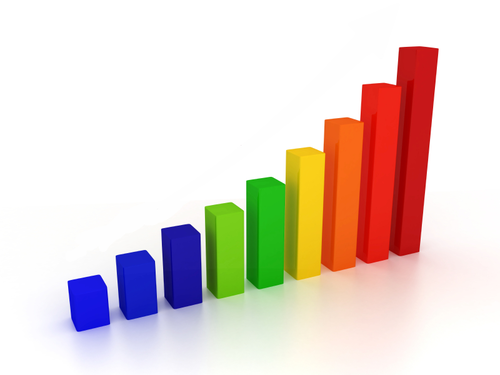
\includegraphics[width=0.5\textwidth]{graph.png}
%   \caption{Grafikon}
% \end{figure}


% % Primer jednostavnije matematičke formule
% Evo i jedan primer matematičke formule: $e^{i\pi} + 1 = 0$. 
% % Primer referisanja na sliku
% Na slici \ref{fig:grafikon} prikazan je jedan grafikon.

% % primer kompleksnije matematičke formule
% $$
% \int_a^b f(x)\ \mathrm{d}x \ =_{def}\ \lim_{\max{\Delta x_k \rightarrow 0}} \sum_{k=1}^n f(x_k^*)\Delta x_k
% $$

% % primer referisanja na poglavlja i strane poglavlja
% Više detalja biće dato u glavi \ref{chp:razrada} na strani \pageref{chp:razrada}.

% % primer liste
% Možemo praviti i nabrajanja:
% \begin{enumerate}
% \item Analiza 1
% \item Linearna algebra
% \item Analitička geometrija
% \item Osnovi programiranja
% \end{enumerate}

% \pangrami

% ------------------------------------------------------------------------------
% \chapter{Opis korišćenih optimizacionih metoda}
% \label{chp:opisMetoda}

% % ------------------------------------------------------------------------------

% % \pangrami

% % \pangrami

% % ------------------------------------------------------------------------------
% U ovom poglavlju biće dat kratak pregled optimizacionih metoda koje su korišćene za rešavanje problema najkraće
% zajedničke nadniske. Te medote su:
% \begin{enumerate}
%   \item Metaheuristika Pretraga Bima
%   \item Heuristička funkcija Većinsko Spajanje
%   \item Heuristička funkcija Težinsko Većinsko Spajanje
% \end{enumerate}
% U nastavku teksta biće opisane pomenute metode, ali samo kao nezavisne celine, algoritam koji kombinuje
% rad ovih metoda biće predstavljen u narednom poglavlju.

% \section{Metaheuristika Pretraga Bima}
% \label{sec:pretragaBima}
% \begin{figure}[!ht]
%   \centering
%   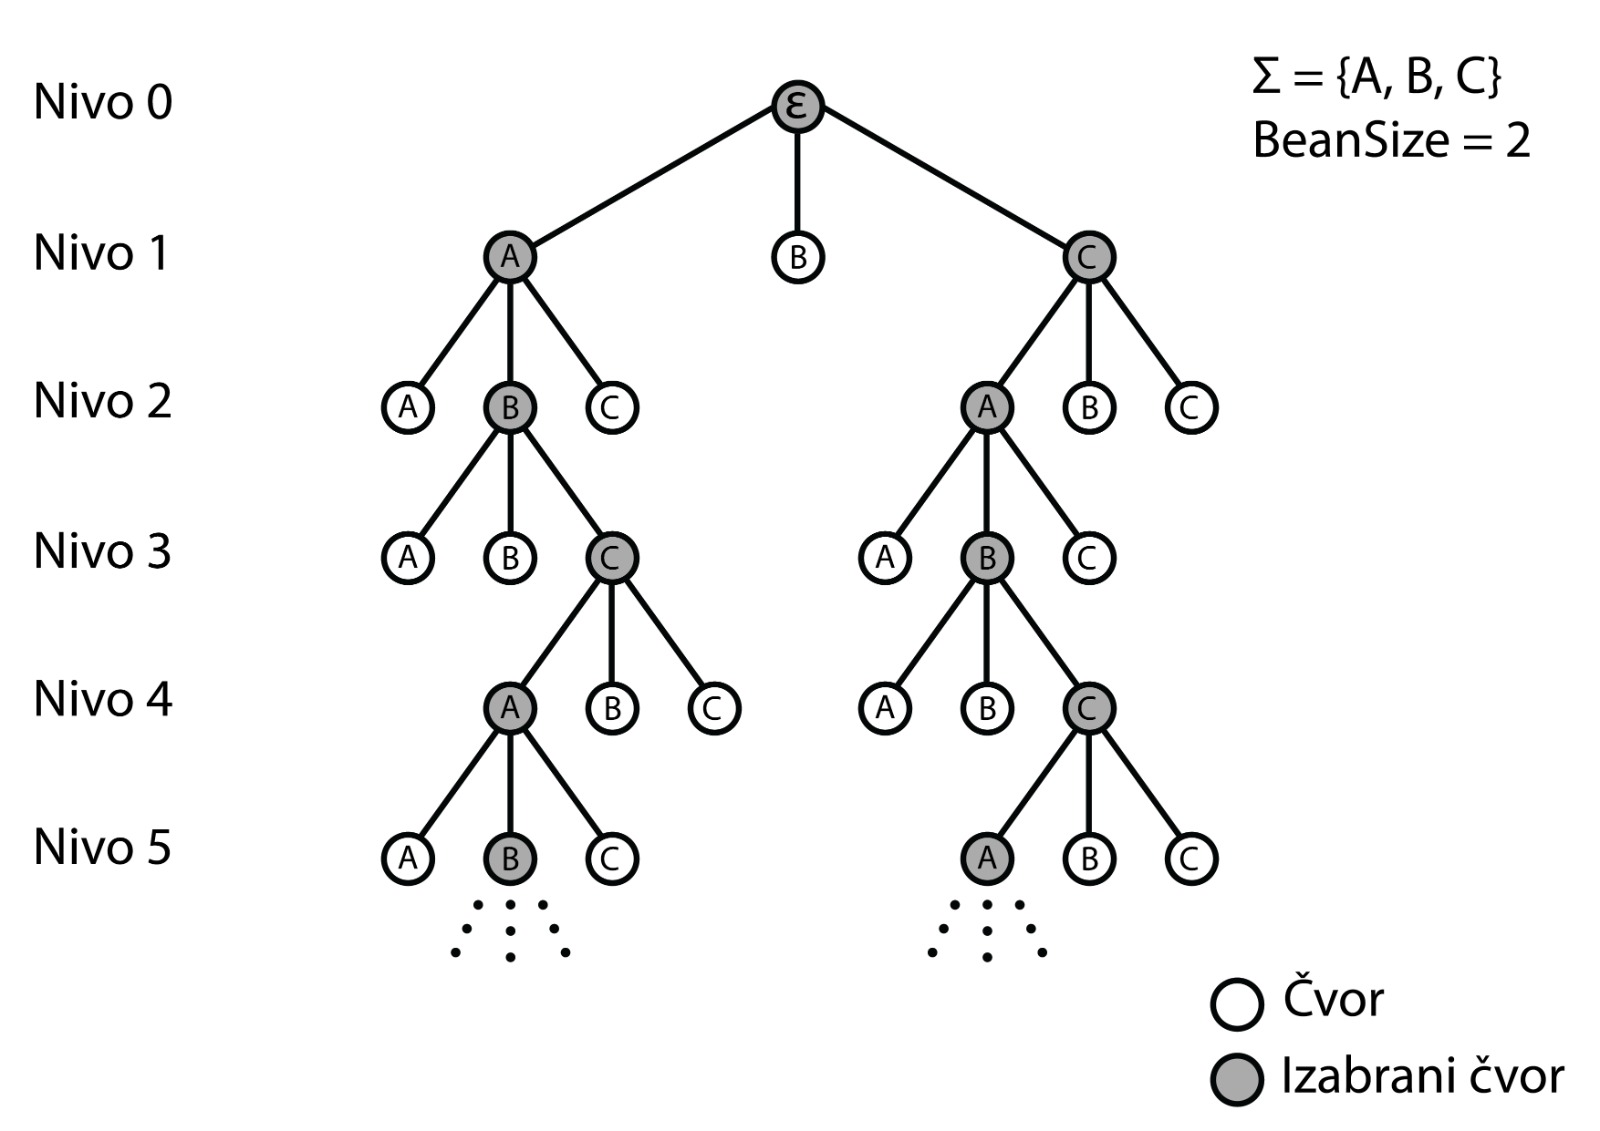
\includegraphics[width=1\textwidth]{Slike/bs2.png}
%   \caption{Šema metaheuristike Pretraga Bima} 
%   \label{fig:pretragaBima}
% \end{figure}
% Sada ćemo predstaviti generalnu ideju Pretrage Bima na kojoj ćemo kasnije izgraditi algoritam za PNZN.
% Pretraga Bima predstavlja metaheuristiku koja je uvedena 1976. godine u oblasti prepoznavanja govora
% (\textit{eng.} speech recognition). Korišćena je u završnim slojevima mnogih modela za
% obradu prirodnog jezika (\textit{eng.} natural language processing models) u donošenju odluke da se izabere najbolji
% izlaz date ciljne promenjive \cite{BSIntroduction}. Pored navedenih primena pretraga bima se intenzivno koristi u sledećeim
% oblastima: kombinatorna optimizacija (\textit{eng.} combinatorial optimization), problemi planiranja (\textit{eng.} scheduling problems),
% problemi rutiranja vozila (\textit{eng.} vehicle routing problems), podešavanje hiperparametara u oblasti mašinskog učenja
% (\textit{eng.} Machine Learning Hyperparameter Tuning), problemi zadovoljenja ograničenja (\textit{eng.} Constraint Satisfaction Problems). 

% Pretraga Bima predstavlja vrstu pretrage grafa u širinu u cilju da
% se pronađe najbolji put od korenog čvora do ciljanog čvora u grafu. Kako bi se složenost izračunavanja držala u
% zadatim granicama, Pretraga Bima evaluira dostignute čvorove na određenom nivou ali bira samo podskup od $\beta$
% čvorova koji najviše obećavaju i sa tim podskupom čvorova napreduje dalje u pretrazi. Izabrani podskup od $\beta$ čvorova
% zvaćemo bim (\textit{eng.} beam) i označavaćemo ga sa $\mathbb{B}$, a $\beta$ parametar ćemo zvati širina bima (\textit{eng.} beam width) \cite{SCSBS}.
% U kontekstu PNZN graf koji pretražujemo $\mathcal{G}=(\mathcal{V},\mathbb{E})$ predstavlja usmeren aciklički graf, a  
% pseudo kod algoritma prikazan je pod Algoritam \ref{alg:bs} i dat u kontekstu problema najkraće
% zajedničke nadniske. 
% \\
% \begin{algorithm}
%   \caption{PretragaBimaPNZN($\Sigma$, $\mathcal{L}$, $\beta$)}
%   \label{alg:bs}
%   \begin{algorithmic}[1]
%   % \Require $n \geq 0$
%   % \Ensure $y = x^n$
%   \State $\mathcal{B} \gets \{ \}$
%   \While{$\textrm{Tačno}$} \Comment{Može postojati uslov izlaska iz petlje pre pronađenog rešenja}
%   \State $\mathcal{B} \gets \textrm{ProširiBim}(\Sigma)$
%   \State $\textrm{OceniBim}(\mathcal{B}, \mathcal{L})$
%   \State $\mathcal{B} \gets \textrm{RedukujBim}(\mathcal{B}, \beta)$
%   % \State \If{x}
%   % \ElsIf{$N$ is odd}
%   \For{$\omega\in\mathcal{B}$}
%     \If{$\textrm{ZajedničkaNadniska}(\omega,\mathcal{L})$}
%     \State \Return $\omega$
%     \EndIf
%   \EndFor
%   \EndWhile
%   \end{algorithmic}
%   \end{algorithm}
% \\
% Algoritam prima tri ulazna parametra: azbuku $\Sigma$, ulazni skup reči $\mathcal{L}$ i širinu bima $\beta$.
% Na početku bim $\mathcal{B}$ predstavlja prazan skup. U svakom koraku algoritma bim se proširuje slovima iz azbuke,
% a zatim se elementi proširenog bima ocenjuje izabranom heurističkom funkcijom. Zatim se vrši odabir $\beta$ čvorova
% sa kojima se dalje nastavlja pretraga, i vrši se provera da li neki čvor u bimu predstavlja rešenje problema,
% ako takav čvor postoji algoritam vraća pronađeno rešenje. Funkcija ProširiBim u prvom koraku popunjava bim slovima
% iz azbuke, a u svakom narednom koraku svako parcijalno rešenje redukovanog bima proširuje dodavajući na njega redom
% slova iz azbuke. Funkcija OceniBim predstavlja heurističku funkciju koja dodeljuje određene vrednosti svakom elementu bima,
% a na osnovu ovih vrednosti funkcija RedukujBim bira $\beta$ parcijalnih rešenja koja imaju najveće vrednosti
% heurističke funkcije. Tokom redukcije bima vrednosti ocena parcijalnih rešenja mogu da se sortiraju tako da redukovani
% bim sadrži $\beta$ najbolje ocenjenih rešenja, ali mogu se koristiti i druge strategije odabira rešenja poput ruletske
% selekcije (\textit{eng.} roulette selection). Funkcija ZajedničkaNadniska vrši proveru da li reč $\omega$
% predstavlja zajedničku nadnisku reči iz skupa $\mathcal{L}$ i jedna njena implementacija će biti opisana u sledećem poglavlju.
% Algoritam se može zaustaviti kada se pronađe prvo rešenje problema, ali mogu se postaviti i drugi uslovi zaustavljanja
% poput broja iteracija petlje (predstavlja dubinu unutar stabla pretrage) ili vremenska ograničenja.

% \section{Heurističke funkcije Većinsko Spajanje i Težinsko Većinsko Spajanje}
% \label{sec:MMiWMM}
% Većinsko Spajanje predstavlja jedan od najpopularnijih algoritama koji rešava PNZN. To je pohlepni algoritam
% koji inkrementalno konstruiše supersekvencu. Najpre se odredi slovo koje se najčešće nalazi na početku reči
% iz skupa $\mathcal{L}$, a zatim se izabrano slovo briše sa početka reči iz $\mathcal{L}$ koje ga sadrže \cite{ProbabilisticBS}.
% Pseudo kod algoritma prikazan je pod Algoritam \ref{alg:mm}.

% \begin{algorithm}
%   \caption{VećinskoSpajanje($\mathcal{L}=\{\omega_{1}, \omega_{2},..., \omega_{m}\}, \Sigma$)}
%   \label{alg:mm}
%   \begin{algorithmic}[1]
%   % \Require $n \geq 0$
%   % \Ensure $y = x^n$
%   \State $\mathcal{S} \gets \varepsilon$ \Comment{supersekvenca}
%   \While{$\sum_{\omega_{i}\in\mathcal{L}}|\omega_{i}| \neq 0$} 
%   \For{$\alpha \in \Sigma$}
%         \State $v(\alpha|\mathcal{S}) \gets \sum_{\omega_{i}\in\mathcal{L},\omega_{i}=\alpha\omega^{'}_{i}}1$
%   \EndFor
%   \State $\beta \gets argmax \{v(\alpha|\mathcal{S})\textrm{ }|\textrm{ }\alpha \in \Sigma \}$
%   \State $\mathcal{L} \gets \mathcal{L}|_{\beta}$
%   \State $\mathcal{S} \gets \mathcal{S}\beta$
%   \EndWhile
%   \State \Return $\mathcal{S}$
%   \end{algorithmic}
%   \end{algorithm}

% Mana Većinskog Spajanja je to što ne može da prepozna globalnu strukturu reči iz skupa $\mathcal{L}$.
% U principu Većinsko spajanje izostavlja činjenicu da reči mogu biti različitih dužina. To dalje 
% znači da će slova sa početka kraćih reči imati veću šansu da budu uklonjena iako algoritam i dalje treba
% da obradi preostale dugačke reči. Iz tog razloga bi skidanje slova sa početka kraćih reči trebalo da bude
% manje prioritetno. Drugim rečima bolje je da se prioritizira skidanje slova sa početka dužih reči.
% To se može postići dodavanjem težine svakom simbolu azbuke u odnosu na dužinu preostalih reči iz $\mathcal{L}$ 
% nakon uklanjanja tog simbola sa početka reči koje počinju tim simbolom. Dakle korak 4 u algoritmu VećinskoSpajanje
% možemo zameniti sa:
% \\
% \\
% \begin{equation}
%   \label{eqn:wmm}
%   v(\alpha|\mathcal{S}) \gets \sum_{\omega_{i}\in\mathcal{L},\omega_{i}=\alpha\omega^{'}_{i}}|\omega^{'}_{i}| 
% \end{equation}
% \\
% \\
% Ovako modifikovan algoritam naziva se Težinsko Većinsko Spajanje i postoje indikacije da na određenim instancama
% problema može da nadmaši algoritam Većinskog Spajana, pogotovo kada nema struktuiranosti unutar skupa $\mathcal{L}$
% ili kada je ta struktuiranost haotična \cite{ProbabilisticBS}.Predstavljena dva algoritma biće korišćena u nastavku
% rada kao heurističke funkcije koje će ocenjivati elemnte bima.

\chapter{Algoritmi za rešavanje problem najkraće zajedničke nadniske}
U ovom poglavlju biće dat pregled sledeća dva algoritama koja su koršćena za rešavanje problema najkraće zajedničke
nadniske:


\begin{enumerate}
  \item Algoritam grananja sa odsecanjem (\textit{eng.} backtracking)
  \item Pretraga Bima (\textit{eng.} Beam Search)
\end{enumerate}
U nastavku teksta biće opisana konstrukcija ova dva algoritma kao i njihove karakteristike.


\section{Algoritam grananja sa odsecanjem}
\label{sec:algGrananjaSaOdsecanjem}
Algoritam grananja sa odsecanjem poboljšava tehniku grube sile tako što vrši provere tokom generisanja
kandidata za rešenja i tako što se odbacuju parcijalno popunjeni kandidati za koje se unapred može utvrditi
da se ne mogu proširiti do optimalnog rešenja problema. Dakle, grananje sa odsecanjem podrazumeva da se tokom
obilaska u dubinu drveta, kojim se predstavlja prostor potencijalnih rešenja odsecaju oni delovi drveta za koje se unapred
može utvrditi da ne sadrže ni jedno rešenje problema tj. da ne sadrže optimalno rešenje, pri čemu se odsecanje vrši
i u čvorovima bliskim korenu koji mogu da sadrže i samo parcijalno popunjene kandidate za rešenja.
Dakle, umesto da se čeka da se tokom pretrage stigne do lista (ili eventualno unutrašnjeg čvora koji predstavlja
nekog kandidata za rešenje) i da se provera zadovoljenosti uslova ili optimalnosti vrši tek tada, prilikom granja sa
odsecanjem provera se vrši u svakom koraku i vrši se provera parcijalno popunjenih rešenja.
Efikasnost ovakvog algoritma uveliko zavisi od kvaliteta kriterijuma na osnovu kojih se vrši odsecanje. Iako obično
složenost najgoreg slučaja ostaje eksponencijalna (kakva je po pravili kod algoritama grube sile), pažljivo odabrani
kriterijumi odsecanja mogu odseći jako velike delove pretrage (koji su često takođe eksponencijalne veličine u odnosu
na dimenzije ulaznog problema) i time značajno ubrzati proces pretrage.

U kontekstu PNZN korišćen je rekurzivni algoritam prikazan pod Algoritam \ref{alg:brutef}.
\begin{algorithm}
  \caption{\textbf{GrananjeSaOdsecanjem($\bm{\omega}$)}}
  \label{alg:brutef}
  \begin{algorithmic}[1]
  % \Require $n \geq 0$
  % \Ensure $y = x^n$
  \State $d \gets |\omega|$ \Comment{$d$ - dužina trenutne reči}
  \If{$(d > maxD) \lor (d \geq nd)$}
      \State \Return
  \EndIf

  \If{$(d \geqslant minD ) \land  \textbf{ZajedničkaNadniska}(\omega)$}
      \State $iDaljeNadniska \gets Ta\textrm{č}no$
      \State $pozicija \gets 0$
      \While{$iDaljeNadniska$} \Comment{optimizacija}
        \If{$\textbf{ZajedničkaNadniska}(\omega[pozicija + 1:])$}
          \State $pozicija \gets pozicija + 1$
        \Else
          \State $iDaljeNadniska = Neta\textrm{č}no$
        \EndIf
      \EndWhile
      \State $nn \gets \omega[pozicija:]$ \Comment{$nn$ - najbolja nadniska}
      \State $nd \gets |nn|$ \Comment{$nd$ - najbolja dužina}
  \EndIf

  \For{$\alpha \in \Sigma$} \Comment{grananje po slovima azbuke}
        \State $\textbf{GrananjeSaOdsecanjem}(\omega\alpha)$
  \EndFor
  \end{algorithmic}
  \end{algorithm}
Algoritam podrazumeva postojanje dve globalne promenjive $minD$ i $maxD$ čije se vrednosti postavljaju pre
poziva algoritma i one označavaju redom minimalnu i maksimalnu dubinu, takođe se podrazumeva da su skupovi $\mathcal{L}$
i $\Sigma$ globalno dostupni u programu. Vrednost promenjive $minD$ postavlja
se na dužinu najkraće reči u $\mathcal{L}$, a vrednost promenjive $maxD$ predstavlja proizvod veličine azbuke
i najduže reči u skupu $\mathcal{L}$ kao što je prikazano u jednačinama \ref{eqn:minD} i \ref{eqn:maxD}
\\
\begin{equation}
  \label{eqn:minD}
  minD=\{min_{\omega\in\mathcal{L}}|\omega|\}
\end{equation}

\begin{equation}
  \label{eqn:maxD}
  maxD=|\Sigma| * L \textrm{, gde } L=\{max_{\omega\in\mathcal{L}}|\omega|\}
\end{equation}
\\
Sada ćemo ova uvedena ograničenja minimalne i maksimalne dubine objasniti na kratkom primeru.
Za instancu PNZN $\mathcal{I}=(\{a,c,t,g\},\{acta,cta,ac\})$ znamo da najkraća zajednička nadniska
ne može biti kraća od dužine najkraće reči u skupu $\mathcal{L}$, jer takva niska ne bi sadržala ni
minimalnu reč a samim time ni ostale reči u $\mathcal{L}$, pa vrednost promenjive $minD=|ac|=2$. Takođe za 
instancu problema $I$ mi sigurno znamo jedno rešenje PNZN. Kako je najduža reč $acta$ dužine 4 
važi da reč $\omega=\underline{actg}_{1}\underline{actg}_{2}\underline{actg}_{3}\underline{actg}_{4}$
sigurno predstavlja jedno rešenje problema, pa važi da $maxD=|\omega|=|\Sigma|*|acta| = 4 * 4 = 16$.

Nakon postavljanja ograničenja dubine, rekurzivni algoritam se poziva
u obliku GrananjeSaOdsecanjem($\varepsilon$) kako bi pretraga u dubinu krenula od prazne reči.
U svakom koraku algoritma vrši se provera da li je dužina trenutne reči $d$ veća od maksimalne dubine ili je veća od
dužine trenutno najbolje pronađene nadniske (na početku $nd=maxD + 1$) i ako jeste vrši se odsecanje tog podstabla u prostoru
pretrage. Ako važi da je dužina trenutne reči $d$ veća od minimalne dubine i pritom važi da reč
$\omega$ predstavlja zajednučku nadnisku reči u skupu $\mathcal{L}$, pronađeno je jedno rešenje PNZN.
Pre ažuriranje vrednosti najbolje nadniske ($nn$) i najbolje dužine ($nd$) pokušava se sa skraćivanjem
reči $\omega$ u cilju dobijanja kraće nadniske, a time i većeg broja odsecanja u prostoru pretrage.
Na primeru gore navedene instance problema $I$, kako se obilazak stabla vrši u dubinu i grananje u svakom
rekurzivnom pozivu počinje prvim slovom azbuke, u ovom slučaju $a$, često se dobijaju rešenja
oblika $\omega=aa...aR$, gde $\omega$ predstavlja rešenje PNZN, ali i $R$ predstavlja rešenje pa stoga
možemo ukloniti prefiks reči $\omega$, sve dok skraćivanjem i dalje dobijamo validno rešenje problema.
Na kraju, vrši se grananje po svim slovima azbuke i rekurzivno poziva algoritam sa argumentom $\omega\alpha$
koji proširuje trenutnu reč $\omega$ novim slovom iz azbuke $\Sigma$. Funkcija $\textrm{ZajedničkaNadniska}(\omega)$ vrši proveru
da li reč $\omega$ predstavlja zajednučku nadnisku reči iz skupa $\mathcal{L}$, i u ovom slučaju se podrazumeva
da je skup $\mathcal{L}$ globalno dostupan. Pseudo kod je dat pod Algoritam \ref{alg:zajNad}. 
U svakom koraku petlje proverava se da li je trenutna reč $s\in\mathcal{L}$ podniska reči $\omega$,
ako nije funkcija vraća $\textrm{Netačno}$, a ako su sve reči podniske reči $\omega$ funkcija vraća $\textrm{Tačno}$.
U suštini važi jednostavna logička formula \ref{eqn:podniskaNadniska}:

\begin{equation}
  \label{eqn:podniskaNadniska}
  \{Podniska(s,\omega) \textrm{ }| \textrm{ } \forall s \in \mathcal{L} \} 
  \Longleftrightarrow 
  \{\omega\succ s \textrm{ }| \textrm{ } \forall s \in\mathcal{L}\} 
\end{equation}
Ako su sve reči iz skupa $\mathcal{L}$ podniske reči $\omega$ onda važi da je $\omega$ nadniska svih reči
iz $\mathcal{L}$ i obrnutno. Pseudo kod funkcije $\textrm{Podniska}(s,\omega)$ dat je pod Algoritam \ref{alg:podNiska}.
Na početku se vrši inicijalizacija promenjivih, $sP$ i $\omega P$ predstavljaju indekse početka reči $s$ i $\omega$,
$sK$ i $\omega K$ redom predstavljaju indekse na kraj reči $s$ i $\omega$.
U svakom koraku petlje vrši se provera da li se stiglo do kraja reči $\omega$, i ako je to slučaj, a prethodno nismo prošli sva
slova reči $s$ znamo da $s$ sigurno nije podniska reči $\omega$. Svaki put kada se vrednosti na pozicijama $sP$ i 
$\omega P$ u rečima $s$ i $\omega$ poklope, oba indeksa inkrementiramo, a u suprotnom napredujemo samo kroz reč
$\omega$ pa inkrementiramo njen indeks $\omega P$. Petlja se završava kada prođemo sva slova reči $s$ i tada znamo
da je $s$ sigurno podniska reči $\omega$.
\\
\begin{algorithm}
  \caption{$\textbf{ZajedničkaNadniska}\bm{(\omega)}$}
  \label{alg:zajNad}
  \begin{algorithmic}[1]
  \For{$s \in \mathcal{L}$}
    \If{$\neg \textbf{Podniska}(s,\omega)$}
    \State \Return $Neta\textrm{č}no$
    \EndIf
  \EndFor
  \State
  \State \Return $Ta\textrm{č}no$
  \end{algorithmic}
  \end{algorithm}

  \begin{algorithm}
    \caption{$\textbf{Podniska}\bm{(s,\omega)}$}
    \label{alg:podNiska}
    \begin{algorithmic}[1]
    \State $sP \gets 0$ \Comment{indeks na početak reči $s$}
    \State $sK \gets |s|$ \Comment{indeks na kraj reči $s$}
    \State $\omega P \gets 0$ \Comment{indeks na početak reči $\omega$}
    \State $\omega K \gets |s|$ \Comment{indeks na kraj reči $\omega$}

    \State
    \While{$sP \neq sK$}
      \If{$\omega P == \omega K$}
        \State \Return $Neta\textrm{č}no$
      \ElsIf{$s[sP] == \omega[\omega P]$}
        \State $sP \gets sP + 1$
        \State $\omega P \gets \omega P + 1$
      \Else
        \State $\omega P \gets \omega P + 1$
      \EndIf
    \EndWhile
    \State
    \State \Return $Ta\textrm{č}no$
    \end{algorithmic}
    \end{algorithm}
Iako algoritam grananja sa odsecanjem u najgorem slučaju ima eksponencijalnu složenost $O(|\Sigma|^{maxD})$
kao i algoritam Iscrpne Pretrage (\textit{eng.} Brute Force), u praksi je prosečno vreme izvršavanja
daleko kraće. Rezultati izvršavanja algoritma grananja sa odsecanjem biće prikazani u sledećem poglavlju.
Ono što je bitno istaći jeste da ovaj algoritam garantuje pronalaženje optimalnog rešenja PNZN, što omogućava
jednostavnu proveru uspešnosti algoritma Pretrage Bima (koji će biti predstavljen u sledećoj sekciji)
na manjim instancam PNZN. S obzirom na eksponencijalnu prirodu ovog algoritma, ne moguće je koristiti ga
za proveru kvaliteta rešenja Pretrage Bima na većim instancama problema, stoga će u te svrhe biti korišćene
nešto sofisticiranije metode koje će biti objašnjene u poglavlju ref.

% \section{Algoritam Pretraga Bima}
% Kao što je već rečeno u sekciji \ref{sec:pretragaBima} Pretraga Bima predstavlja metaheuristiku
% koja graf koji predstavlja prostor rešenja problema obilazi u širinu. Metaparametar $\beta$
% koji nazivamo širina bima kontroliše broj elemenata unutar Bima koji označavamo sa $\mathcal{B}$.
% Zapravo podešavanjem vrednosti parametra $\beta$ kontrolišemo broj čvorova unutar grafa sa kojima
% nastavljamo grananje, a time i ograničavamo složenost izračunavanja na svakom nivou. Odabir čvorova
% koji najviše obećavaju na svakom nivou usmerava pretragu ka pronalasku rešenja i odabir će
% se vršiti heurističkim funkcijama opisanim u sekciji \ref{sec:MMiWMM}. Nažalost ovaj algoritam
% ne garantuje pronalak optimalnog rešenja, ali za razumne vrednosti metaparametra $\beta$
% daje prihvatljivo vreme izvršavanja u realnim uslovima, pa čak i na velikim instancama PNZN.

\section{Pretraga Bima}
\label{sec:pretragaBima}
\begin{figure}[!ht]
  \centering
  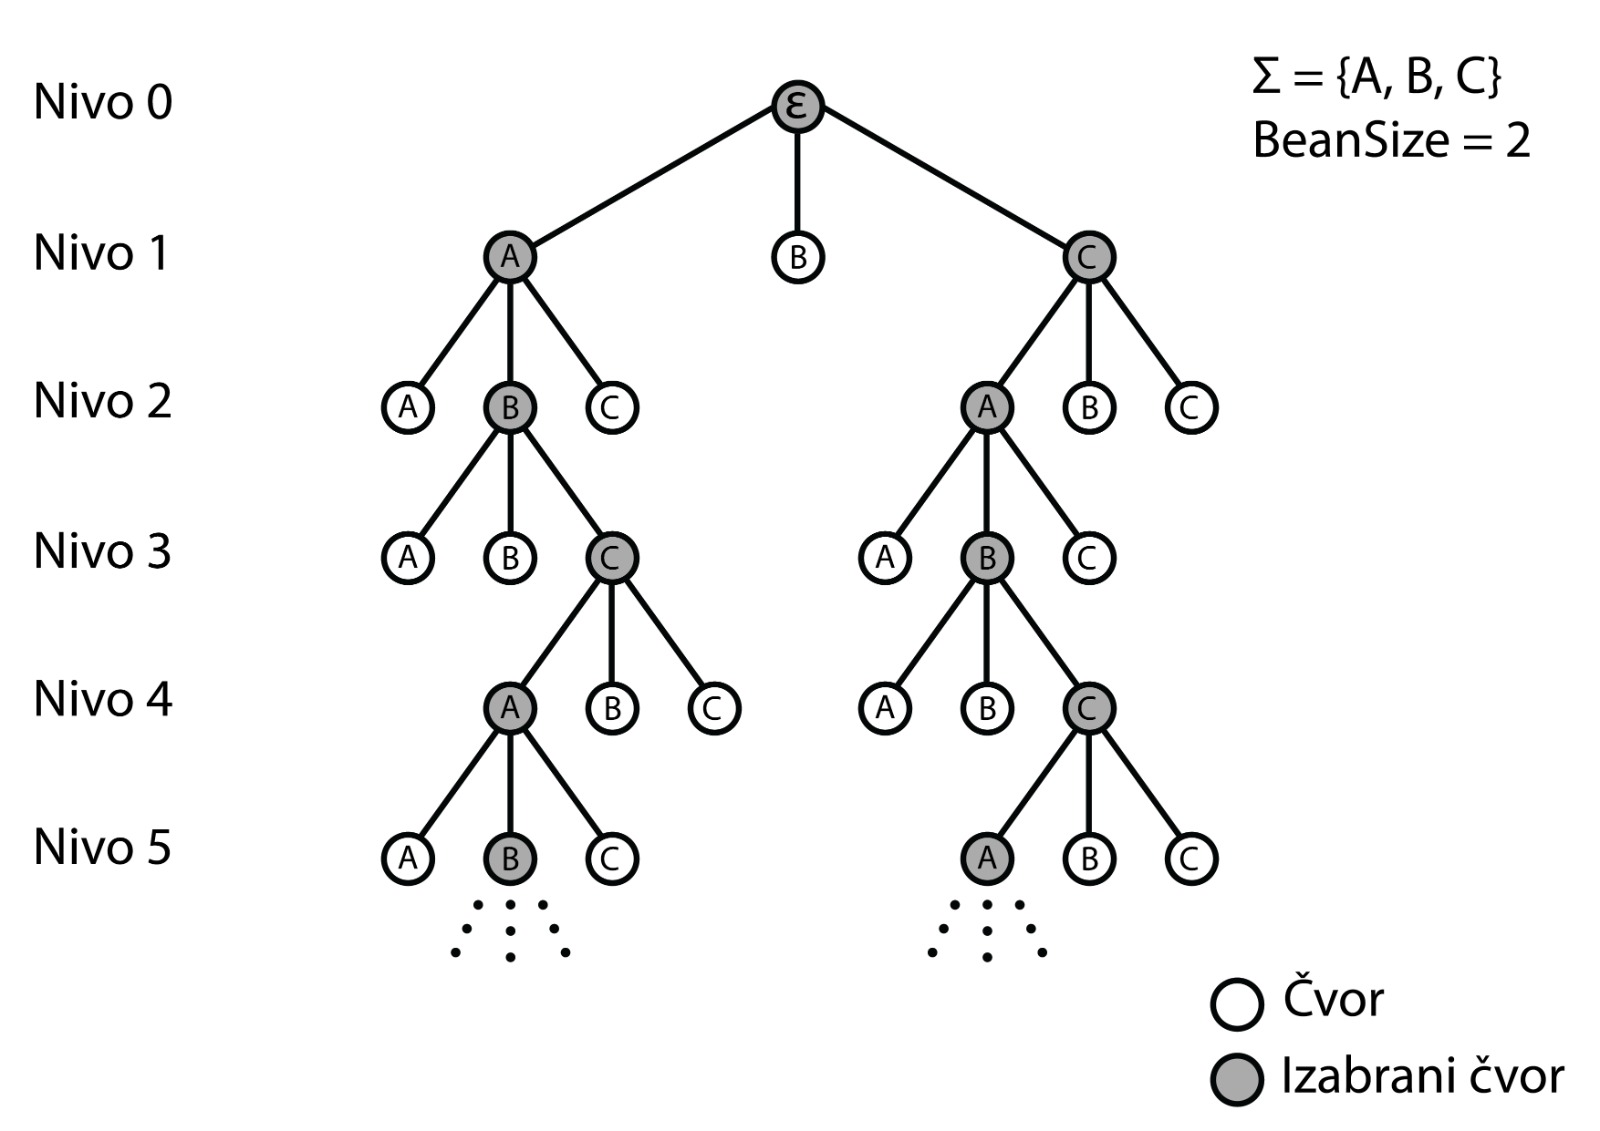
\includegraphics[width=1\textwidth]{Slike/bs2.png}
  \caption{Šema metaheuristike Pretraga Bima} 
  \label{fig:pretragaBima}
\end{figure}
% Sada ćemo predstaviti generalnu ideju Pretrage Bima na kojoj ćemo kasnije izgraditi algoritam za PNZN.
Pretraga Bima predstavlja metaheuristiku koja je uvedena 1976. godine u oblasti prepoznavanja govora
(\textit{eng.} speech recognition). Korišćena je u završnim slojevima mnogih modela za
obradu prirodnog jezika (\textit{eng.} natural language processing models) u donošenju odluke da se izabere najbolji
izlaz date ciljne promenjive \cite{BSIntroduction}. Pored navedenih primena pretraga bima se intenzivno koristi u sledećeim
oblastima: kombinatorna optimizacija (\textit{eng.} combinatorial optimization), problemi planiranja (\textit{eng.} scheduling problems),
problemi rutiranja vozila (\textit{eng.} vehicle routing problems), podešavanje hiperparametara u oblasti mašinskog učenja
(\textit{eng.} Machine Learning Hyperparameter Tuning), problemi zadovoljenja ograničenja (\textit{eng.} Constraint Satisfaction Problems). 

Pretraga Bima predstavlja vrstu pretrage grafa u širinu u cilju da
se pronađe najbolji put od korenog čvora do ciljanog čvora u grafu. Kako bi se složenost izračunavanja držala u
zadatim granicama, Pretraga Bima evaluira dostignute čvorove na određenom nivou ali bira samo podskup od $\beta$
čvorova koji najviše obećavaju i sa tim podskupom čvorova napreduje dalje u pretrazi. Izabrani podskup od $\beta$ čvorova
zvaćemo bim (\textit{eng.} beam) i označavaćemo ga sa $\mathbb{B}$, a $\beta$ parametar ćemo zvati širina bima (\textit{eng.} beam width) \cite{SCSBS}.
U kontekstu PNZN graf koji pretražujemo $\mathcal{G}=(\mathcal{V},\mathbb{E})$ predstavlja usmeren aciklički graf, 
a pseudo kod algoritma je prikazan pod Algoritam \ref{alg:bs}.

Kao i u prethodno opisanom algoritmu podrazumeva se da je promenjiva $maxD$ globalno dostupna,
kao i skupovi $\mathcal{L}$ i $\Sigma$. Svaki element skupa $\mathcal{B}$ predstavlja objekat koji
sadrži parcijalnu reč, heurističku ocenu i pozicije.
Parcijalna reč predstavlja put od korena do nekog čvora unutar stabla pretrage, 
heuristička ocena predstavlja ocenu ove reči od strane heurističke funkcije, a pozicije predstavljaju
niz koji oznčava pozicije do kojih se stiglo unutar skupa $\mathcal{L}$.
Pri proširivanju skupa $\mathcal{B}$ slovima iz azbuke $\Sigma$, dobijaju se novi
elementi čija je parcijalna reč proširena novododatim slovom. Od jednog elementa
dobijamo maksimalno $|\Sigma|$ novih, što znači da u svakom koraku algoritma dobijamo
maksimalno $\beta * |\Sigma|$ novih elemenata od kojih je potrebno izabrati $\beta$ 
elemenata. Heurističke funkcije, koje će biti predstavljene u narednom podpoglavlju,
za dati niz pozicija računaju ocene za svako slovo azbuke. Recimo ako je data azbuka 
$\Sigma=\{a, c, t, g\}$ i skup $\mathcal{L}=\{actt,gcac,ctga\}$ 

pohlepno vrše ocenu slova na taj način što 
ocenjuju slova u zavisnosti od pozicija unutar skupa $\mathcal{L}$, zapravo bitna su
početna slova reči 

S obzirom na pohlepnu prirodu heurističkih funkcija koje su detaljno objašnjene
u sledećem podpoglavlju, svaki element bima  u svakom koraku algortima vrši se ocena slova iz azbuke
u zavisnosti od pozicija u skupu $\mathcal{L}$ do kojih je element bima stigao, zapravno
parcijalna reč koju taj element sadrži.
tako da se na parcijalno rešenje elementa bima 

Algoritam \ref{alg:bs} inkrementalno gradi nadnisku,
tako što u svakom koraku glavne petlje, za svaki element bima najpre izračunava
vrednost heurističke funkcije $\textbf{H}$, i ovde je napravljeno malo odstupanje
od klasičnog algoritma pretrage bima koji prvo proširuje bim a zatim vrši ocenu elemenata 
heurističkom funkcijom. Zboj prirode predloženih funkcija

Iz tog razloga je inicijalni korak pretrage bima obrađen izvan glavne petlje.
\\
\begin{algorithm}
  \caption{\textbf{PretragaBimaPNZN()}}
  \label{alg:bs}
  \begin{algorithmic}[1]
  % \Require $n \geq 0$
  % \Ensure $y = x^n$
  \State $b1 \gets \{ \}$
  \State $b2 \gets \{ \}$
  \State $prona\textrm{đ}enaNadniska \gets Neta\textrm{č}no$
  \State
  \State $te\textrm{ž}ine \gets \textbf{H}\textrm{([0,...,0])}$
  \State
  \For{$\alpha\in\Sigma$}
    \State $te\textrm{ž}inaSlova \gets 0$
    \For{$t\in te\textrm{ž}ine$}
      \If{$\alpha == t\textrm{.}slovo$}
        \State $te\textrm{ž}inaSlova \gets t\textrm{.}vrednost$
      \EndIf
    \EndFor
    \State $element \gets \{\alpha\textrm{, }te\textrm{ž}inaSlova \textrm{, [0,...,0]}\}$
    \State $b1\textrm{.}dodaj(element)$
  \EndFor
  \State
  \State $b1 \gets \textbf{RedukujBim}(b1\textrm{, }prona\textrm{đ}enaNadniska)$
  \State $dubina \gets 0$
  \State
  \While{$\neg prona\textrm{đ}enaNadniska \land dubina < maxD$} 
    \For{$s\in b1$}
      \State $te\textrm{ž}ine \gets \textbf{H}(s.pozicije)$
      \State
      \If{$te\textrm{ž}ine[0].vrednost == 0$}
        \State $\textbf{SkiniPreostalaSlova}()$
        \State $prona\textrm{đ}enaNadniska \gets Ta\textrm{č}no$
        \State \textbf{break}
      \EndIf
      \State
      \For{$\alpha\in\Sigma$}
        \State $te\textrm{ž}inaSlova \gets 0$
        \For{$t\in te\textrm{ž}ine$}
          \If{$\alpha == t.slovo$}
            \State $te\textrm{ž}inaSlova \gets t.vrednost$
          \EndIf
        \EndFor
      \State $element \gets \{(s.re\textrm{č})\alpha\textrm{, }s.hvrednost + te\textrm{ž}inaSlova\textrm{, }s.pozicije\}$
      \State $b2\textrm{.}dodaj(element)$
      \EndFor
    \EndFor
    \State
    \State $b1\textrm{.}obri\textrm{š}i()$
    \State $b1 \gets \textbf{RedukujBim}(b2\textrm{, }prona\textrm{đ}enaNadniska)$
    \State $b2\textrm{.}obri\textrm{š}i()$
    \State $dubina \gets dubina + 1$
  \EndWhile
  \end{algorithmic}
  \end{algorithm}
\\
\\
\begin{algorithm}
  \caption{$\textbf{RedukujBim}\bm{(\mathcal{B}\textbf{, }prona\textbf{đ}enaNadniska)}$}
  \label{alg:redukujbim}
  \begin{algorithmic}[1]
    \If{$\mathcal{B}.veli\textrm{č}ina() \leqslant \beta$}
      \For{$e \in \mathcal{B}$}
        \State $\textbf{A\textrm{ž}urirajPozicije}(e)$
          \If{$\textbf{ZajedničkaNadniska}(e.re\textrm{č})$}
            \State $nn \gets s.re\textrm{č}$ \Comment{$nn$ - najbolja nadniska}
            \State $nd \gets |nn|$ \Comment{$nd$ - najbolja dužina}
            \State $prona\textrm{đ}enaNadniska \gets Ta\textrm{č}no$
          \EndIf
      \EndFor
      \State \Return $\mathcal{B}$
    \EndIf
    \State
    \State $\textbf{Promešaj}(\mathcal{B})$
    \State $\textbf{Sortiraj}(\mathcal{B})$
    \State $\mathcal{B}\textbf{p} \gets \{ \}$
    \State
    \For{$i=0 \to \beta$}
      \State $\textbf{A\textrm{ž}urirajPozicije}(\mathcal{B}[i])$
      \If{$\textbf{ZajedničkaNadniska}(\mathcal{B}[i].re\textrm{č})}$
            \State $nn \gets \mathcal{B}[i].re\textrm{č}$
            \State $nd \gets |nn|$ 
            \State $prona\textrm{đ}enaNadniska \gets Ta\textrm{č}no$
      \EndIf
      \State $\mathcal{B}\textbf{p}\textrm{.}dodaj(\mathcal{B}[i])$
    \EndFor
    \State
    \State $\mathcal{B}.obri\textrm{š}i()$
    \State \Return $\mathcal{B}\textbf{p}$
  \end{algorithmic}
  \end{algorithm}
\\
\\
\begin{algorithm}
  \caption{$\textbf{AžurirajPozicije}\bm{(element)}$}
  \label{alg:azurirajPozicije}
  \begin{algorithmic}[1]
    \State $poslednjeDodatoSlovo \gets element.re\textrm{č}[element.re\textrm{č}.du\textrm{ž}ina() - 1]$
    \State
    \For{$i=0 \to \mathcal{L}.veli\textrm{č}ina()$}
      \If{$\mathcal{L}[i][element.pozicije[i]] == poslednjeDodatoSlovo$}
            \State $element.pozicije[i] \gets element.pozicije[i] + 1$
      \EndIf
    \EndFor
  \end{algorithmic}
  \end{algorithm}
\\
% Algoritam prima tri ulazna parametra: azbuku $\Sigma$, ulazni skup reči $\mathcal{L}$ i širinu bima $\beta$.
% Na početku bim $\mathcal{B}$ predstavlja prazan skup. U svakom koraku algoritma bim se proširuje slovima iz azbuke,
% a zatim se elementi proširenog bima ocenjuje izabranom heurističkom funkcijom. Zatim se vrši odabir $\beta$ čvorova
% sa kojima se dalje nastavlja pretraga, i vrši se provera da li neki čvor u bimu predstavlja rešenje problema,
% ako takav čvor postoji algoritam vraća pronađeno rešenje. Funkcija ProširiBim u prvom koraku popunjava bim slovima
% iz azbuke, a u svakom narednom koraku svako parcijalno rešenje redukovanog bima proširuje dodavajući na njega redom
% slova iz azbuke. Funkcija OceniBim predstavlja heurističku funkciju koja dodeljuje određene vrednosti svakom elementu bima,
% a na osnovu ovih vrednosti funkcija RedukujBim bira $\beta$ parcijalnih rešenja koja imaju najveće vrednosti
% heurističke funkcije. Tokom redukcije bima vrednosti ocena parcijalnih rešenja mogu da se sortiraju tako da redukovani
% bim sadrži $\beta$ najbolje ocenjenih rešenja, ali mogu se koristiti i druge strategije odabira rešenja poput ruletske
% selekcije (\textit{eng.} roulette selection). Funkcija ZajedničkaNadniska vrši proveru da li reč $\omega$
% predstavlja zajedničku nadnisku reči iz skupa $\mathcal{L}$ i jedna njena implementacija će biti opisana u sledećem poglavlju.
% Algoritam se može zaustaviti kada se pronađe prvo rešenje problema, ali mogu se postaviti i drugi uslovi zaustavljanja
% poput broja iteracija petlje (predstavlja dubinu unutar stabla pretrage) ili vremenska ograničenja.

\subsection{Heurističke funkcije Većinsko Spajanje i Težinsko Većinsko Spajanje}
\label{sec:mmiwmm}
Većinsko Spajanje predstavlja jedan od najpopularnijih algoritama koji rešava PNZN. To je pohlepni algoritam
koji inkrementalno konstruiše supersekvencu. Najpre se odredi slovo koje se najčešće nalazi na početku reči
iz skupa $\mathcal{L}$, a zatim se izabrano slovo briše sa početka reči iz $\mathcal{L}$ koje ga sadrže \cite{ProbabilisticBS}.
Pseudo kod algoritma prikazan je pod Algoritam \ref{alg:mm}.

\begin{algorithm}
  \caption{\textbf{VećinskoSpajanje($pozicije$)}}
  \label{alg:mm}
  \begin{algorithmic}[1]
  % \Require $n \geq 0$
  % \Ensure $y = x^n$
  \State $te\textrm{ž}ine \gets \{\alpha \in \Sigma\textrm{, }[0,...,0] \}$ \Comment{inicijalizacija težina}
  \State
  \For{$i=0 \to \mathcal{L}.veli\textrm{č}ina()$}
    \If{$pozicije[i] \leq (\mathcal{L}[i].du\textrm{ž}ina() - 1)$}
      \For{$t \in te\textrm{ž}ine$}
        \If{$t.slovo == \mathcal{L}[i][pozicije[i]]$}
          \State $t.vrednost \gets t.vrednost + 1$
        \EndIf 
      \EndFor
    \EndIf 
  \EndFor
  \State
  \State $\textbf{Promešaj}(te\textrm{ž}ine)$
  \State $\textbf{Sortiraj}(te\textrm{ž}ine)$
  \State
  \State \Return $te\textrm{ž}ine$
  \end{algorithmic}
  \end{algorithm}

Mana Većinskog Spajanja je to što ne može da prepozna globalnu strukturu reči iz skupa $\mathcal{L}$.
U principu Većinsko spajanje izostavlja činjenicu da reči mogu biti različitih dužina. To dalje 
znači da će slova sa početka kraćih reči imati veću šansu da budu uklonjena iako algoritam i dalje treba
da obradi preostale dugačke reči. Iz tog razloga bi skidanje slova sa početka kraćih reči trebalo da bude
manje prioritetno. Drugim rečima bolje je da se prioritizira skidanje slova sa početka dužih reči.
To se može postići dodavanjem težine svakom simbolu azbuke u odnosu na dužinu preostalih reči iz $\mathcal{L}$ 
nakon uklanjanja tog simbola sa početka reči koje počinju tim simbolom. Dakle korak 4 u algoritmu VećinskoSpajanje
možemo zameniti sa:
\\
\\
\begin{equation}
  \label{eqn:wmm}
  v(\alpha|\mathcal{S}) \gets \sum_{\omega_{i}\in\mathcal{L},\omega_{i}=\alpha\omega^{'}_{i}}|\omega^{'}_{i}| 
\end{equation}
\\
\\
Ovako modifikovan algoritam naziva se Težinsko Većinsko Spajanje i postoje indikacije da na određenim instancama
problema može da nadmaši algoritam Većinskog Spajana, pogotovo kada nema struktuiranosti unutar skupa $\mathcal{L}$
ili kada je ta struktuiranost haotična \cite{ProbabilisticBS}.Predstavljena dva algoritma biće korišćena u nastavku
rada kao heurističke funkcije koje će ocenjivati elemnte bima.

% \lstinputlisting[caption=Sample Code Listing C++, label={lst:listing-cpp}, language=C++]{./code1.cpp}
% ------------------------------------------------------------------------------
% \pangrami

% \pangrami

% ------------------------------------------------------------------------------
% Literatura
% ------------------------------------------------------------------------------
\literatura

% ==============================================================================
% Završni deo teze i prilozi
\backmatter
% ==============================================================================

% ------------------------------------------------------------------------------
% Biografija kandidata
\begin{biografija}
  \textbf{Vuk Stefanović Karadžić} (\emph{Tršić,
    26. oktobar/6. novembar 1787. — Beč, 7. februar 1864.}) bio je
  srpski filolog, reformator srpskog jezika, sakupljač narodnih
  umotvorina i pisac prvog rečnika srpskog jezika.  Vuk je
  najznačajnija ličnost srpske književnosti prve polovine XIX
  veka. Stekao je i nekoliko počasnih mastera.  Učestvovao je u
  Prvom srpskom ustanku kao pisar i činovnik u Negotinskoj krajini, a
  nakon sloma ustanka preselio se u Beč, 1813. godine. Tu je upoznao
  Jerneja Kopitara, cenzora slovenskih knjiga, na čiji je podsticaj
  krenuo u prikupljanje srpskih narodnih pesama, reformu ćirilice i
  borbu za uvođenje narodnog jezika u srpsku književnost. Vukovim
  reformama u srpski jezik je uveden fonetski pravopis, a srpski jezik
  je potisnuo slavenosrpski jezik koji je u to vreme bio jezik
  obrazovanih ljudi. Tako se kao najvažnije godine Vukove reforme
  ističu 1818., 1836., 1839., 1847. i 1852.
\end{biografija}
% ------------------------------------------------------------------------------

\end{document}
